\documentclass[11pt]{article}

\usepackage[margin=0.9in]{geometry}
\usepackage[T1]{fontenc}
\usepackage{lmodern}
\usepackage{microtype}
\usepackage{amsmath,amssymb}
\usepackage{booktabs}
\usepackage{graphicx}
\usepackage{caption}
\usepackage{subcaption}
\usepackage{placeins}
\usepackage{titlesec}
\usepackage{enumitem}
\usepackage{array}
\usepackage[colorlinks=true,linkcolor=black,citecolor=black,urlcolor=blue]{hyperref}

\graphicspath{{../outputs/report/}}
\captionsetup{font=small,skip=4pt,justification=centering}
\titlespacing*{\section}{0pt}{1.2ex plus 0.2ex}{0.5ex}
\titlespacing*{\subsection}{0pt}{0.9ex plus 0.2ex}{0.35ex}
\setlength{\parskip}{0.35em}
\setlength{\parindent}{0pt}
\setlist[itemize]{nosep,leftmargin=1.25em}
\newcolumntype{L}[1]{>{\raggedright\arraybackslash}p{#1}}

\title{\vspace{-1.3em}Technical Signal Discovery in Daily OHLCV Data\\
\large A Walk-Forward Comparison with Reversal and Momentum}
\author{Ritvik Verma \and Tate Gilbertson \and Neel Padhye \and Ahmad Mohammad}
\date{FINM 33100 \textperiodcentered\ Summer 2026}

\begin{document}
\maketitle
\vspace{-1.7em}

\begin{abstract}
We compare simple reversal and momentum signals with a broad library of
OHLCV technical features for U.S.\ equities. Four elastic-net specifications
are evaluated at one- and five-day horizons in yearly walk-forward tests from
2013 through 2025. The baseline and its interaction extension attain the
largest average rank correlations, while the technical specifications produce
greater separation between the extreme deciles. Pruning 103 covered features
to 85 has little effect on out-of-sample results. Predictability is small,
varies materially across years, and is reported before transaction costs.
\end{abstract}

\section{Introduction}

Daily prices and volume support a large number of technical signals. Many are
different transformations of the same recent path, so a large library can
contain more redundancy than independent information. Kakushadze's formulaic
alphas make this issue explicit: the formulas are diverse in appearance, yet
often combine the same primitives---returns, ranges, volume, ranks, delays,
and rolling correlations \cite{kakushadze}.

This study asks how broad technical specifications compare with a simple
three-signal benchmark at one- and five-day horizons. The benchmark contains
one-day reversal, five-day reversal, and 12--1 momentum. The technical library
contains 90 implementable formulaic alphas and 15 conventional OHLCV signals.
We compare the benchmark, a benchmark with pairwise interactions, a
target-blind pruned library, and the full covered library. All four
specifications use the same elastic-net estimator and yearly walk-forward
design.

The comparison separates two questions. Information coefficient (IC) measures
the quality of the full cross-sectional ranking. A decile portfolio measures
whether the ranking is useful at the two tails. The experiments show that
these criteria need not agree. This difference, together with the stability of
the selected coefficients across years, is the main empirical result.

\section{Data and Signal Construction}

\subsection{Panel and prediction target}

The course OHLCV panel contains the largest 1{,}000 U.S.\ equities by
month-end market capitalization from February 2001 through December 2025.
Securities are identified by CRSP \texttt{permno}. After removing rows with a
missing close or market capitalization, the sample contains 6.25 million
security-days and 3{,}253 securities. The daily cross-section has a median of
998 names.

Signals use information dated $t$ to predict the split-adjusted close-to-close
price return
\begin{equation}
 y^{(h)}_{i,t}=\frac{C_{i,t+h}}{C_{i,t}}-1,
 \qquad h\in\{1,5\}.
 \label{eq:target}
\end{equation}
The panel's CRSP \texttt{ret} field is backward-looking and includes
distributions. A separate audit finds that \texttt{ret} and the corresponding
close-to-close return differ by less than one basis point on 99.0\% of
observations. Equation~\eqref{eq:target} therefore measures price
appreciation rather than total return. This differs from the project brief's
preferred construction from compounded \texttt{ret}; the implications are
discussed in Section~\ref{sec:limitations}.

Date gaps longer than ten calendar days start a new listing segment. Targets
and rolling features are set to missing whenever their windows cross a segment
boundary. This prevents an exit and later re-entry from being treated as
adjacent trading days. A true VWAP field is unavailable, so formulas requiring
VWAP use the daily typical price $(H+L+C)/3$.

\subsection{Baseline signals}

Short-horizon reversal is the contrarian hypothesis that recent losers tend
to outperform recent winners over the next few sessions
\cite{jegadeesh,lehmann}. For lookback $k$,
\begin{equation}
 \operatorname{Rev}^{(k)}_{i,t}
 =-\left(\frac{C_{i,t}}{C_{i,t-k}}-1\right),
 \qquad k\in\{1,5\}.
 \label{eq:reversal}
\end{equation}
A stock that lost 4\% over the lookback receives a reversal signal of
$+0.04$; a 4\% winner receives $-0.04$. Larger values therefore identify
recent losers. The third baseline signal is 12--1 momentum,
\begin{equation}
 \operatorname{Mom}^{(12,1)}_{i,t}
 =\frac{C_{i,t-21}}{C_{i,t-252}}-1,
\end{equation}
which omits the most recent month. The interaction specification adds the
three pairwise products of cross-sectionally ranked baseline signals.

\subsection{Technical library}

Of the 101 formulaic alphas, 90 can be constructed from the course panel.
Four formulas require subindustry, three require sector, and four reduce to
identities. Two-digit SIC is used for the alphas defined at the industry
level. The additional 15 signals cover intraday price shape, reversal and
momentum at other lookbacks, volatility, unusual volume, Amihud illiquidity,
and distance from the 52-week high. Appendix~\ref{app:features} records the
complete implementation set.

\section{Empirical Design}

\subsection{Model specifications}

Table~\ref{tab:models} defines the four predeclared comparisons. The technical
models are competing specifications: their design matrices do not include the
three baseline variables.

\begin{table}[ht]
\centering
\caption{Model specifications. Each is estimated separately at the one- and
five-day horizons.}
\label{tab:models}
\small
\begin{tabular}{@{}llL{8.2cm}@{}}
\toprule
Label & Name & Predictors \\
\midrule
A & Baseline & One-day reversal, five-day reversal, 12--1 momentum \\
B & Baseline + interactions & Baseline plus its three pairwise rank products \\
C & Pruned technicals & 85 technical features retained by the frozen
correlation filter \\
D & Full technicals & 103 technical features surviving the coverage screen \\
\bottomrule
\end{tabular}
\end{table}

The pruning sample is 2001--2010 and is excluded from subsequent model
estimation. Features with less than 20\% finite coverage are removed first,
leaving 103 candidates. We then compute the Spearman correlation between each
pair within every date and average those correlations through time. Starting
with the pair having the largest absolute correlation, the feature with the
larger mean absolute correlation to the remaining library is removed until
$|\rho|<0.7$ for every pair. This leaves 85 features. Thresholds of 0.6 and
0.8 retain 76 and 92 features, respectively; the prediction target is absent
from every step.

All features are converted each date to percentile ranks and linearly mapped
to $(-1,1]$. Missing ranks are assigned zero, the cross-sectional midpoint.
This transformation makes coefficients comparable across formulas and limits
the influence of extreme raw alpha values.

\subsection{Elastic net and tuning}

The elastic net combines variable selection with ridge shrinkage
\cite{zouhastie}. For each fold it solves
\begin{equation}
 \min_{\beta_0,\beta}
 \frac{1}{2n}\sum_{j=1}^{n}
 \left(y_j-\beta_0-x_j^\top\beta\right)^2
 +\alpha\left[
 \lambda\|\beta\|_1+\frac{1-\lambda}{2}\|\beta\|_2^2
 \right].
 \label{eq:enet}
\end{equation}
The $\ell_1$ component sets weak coefficients to zero; the $\ell_2$
component stabilizes groups of correlated signals. This combination is
suited to a technical library in which many columns share inputs and
lookback windows.

The mixing parameter is selected from
$\lambda\in\{0.1,0.3,0.5,0.7,0.9,1.0\}$. For each value, a
training-derived path of 30 penalties runs from $\alpha_{\max}$, at which all
slopes are zero, to $10^{-4}\alpha_{\max}$. Validation mean squared error
selects $(\alpha,\lambda)$. The selected pair is then refit on train plus
validation. Figure~\ref{fig:tuning} in the appendix shows that this procedure
selects both sparse and dense models, including several all-zero folds.

\subsection{Walk-forward validation and evaluation}

For test year $Y$, training uses all model-sample years before $Y-1$,
validation uses $Y-1$, and testing uses $Y$:
\begin{center}
\small
\begin{tabular}{ccc}
\toprule
Train & Validation & Test \\
\midrule
$2011,\ldots,Y-2$ & $Y-1$ & $Y$ \\
fit path & select $(\alpha,\lambda)$ & evaluate once \\
\bottomrule
\end{tabular}
\end{center}
The first test year is 2013. Five dates are purged from the end of both
training and validation so that a five-day target cannot cross into the next
block.

On each test date, rank IC is
\begin{equation}
 \operatorname{IC}_t
 =\operatorname{Spearman}_i(\widehat y_{i,t},y_{i,t}).
\end{equation}
The annual IC is the average over dates in that test year. If validation
selects an all-zero model, every prediction is identical and IC is undefined.
We report both the mean over active years and an all-fold mean that assigns
zero to null folds.

Stocks are also sorted into ten equal-weight portfolios by predicted return.
The 100\%-gross long-short return is
\begin{equation}
 r^{LS}_t=\tfrac12(r_{10,t}-r_{1,t}).
 \label{eq:ls}
\end{equation}
One-day portfolios form daily. Five-day portfolios form on every fifth
trading date and use $\sqrt{252/5}$ for annualization. Sharpe is calculated
over the complete non-overlapping formation series, not as an average of
annual Sharpes. Appendix~\ref{app:offset} reports all five possible formation
offsets. Returns are gross of costs.

\section{Results}

\subsection{Overall comparison}

Table~\ref{tab:comparison} reports the complete scorecard: all four
specifications at both horizons. Active IC conditions on a non-null fold; all-fold IC assigns zero
to a null fold. The spread column is the mean return of
Equation~\eqref{eq:ls} in basis points per formation period.

\begin{table}[ht]
\centering
\caption{Out-of-sample comparison, 2013--2025. Sharpe ratios use the full
non-overlapping formation series and are gross of costs.}
\label{tab:comparison}
\small
\begin{tabular}{@{}lcccccc@{}}
\toprule
Specification & $h$ & Active IC & Active & All-fold IC & Spread (bp) & Sharpe \\
\midrule
Baseline & 1d & 0.0102 & 8/13 & 0.0063 & 0.27 & 0.08 \\
Baseline & 5d & 0.0052 & 8/13 & 0.0032 & $-1.90$ & $-0.12$ \\
Baseline + interactions & 1d & 0.0109 & 9/13 & 0.0076 & 0.41 & 0.13 \\
Baseline + interactions & 5d & 0.0052 & 8/13 & 0.0032 & $-0.85$ & $-0.05$ \\
Pruned technicals & 1d & 0.0079 & 10/13 & 0.0061 & 1.56 & 0.63 \\
Pruned technicals & 5d & 0.0041 & 10/13 & 0.0032 & 1.78 & 0.12 \\
Full technicals & 1d & 0.0081 & 10/13 & 0.0062 & 1.52 & 0.61 \\
Full technicals & 5d & 0.0042 & 9/13 & 0.0029 & 1.67 & 0.11 \\
\bottomrule
\end{tabular}
\end{table}

The benchmark and interaction specifications deliver the largest active-year
ICs at both horizons. Once null folds are included as zero-signal years, the
one-day ICs are similar across the baseline and technical specifications.
Adding baseline interactions produces only a small change. The technical
models have lower rank correlation over active years but larger extreme-decile
spreads. Thus the main distinction is between average ordering and tail
separation rather than a uniform improvement in prediction.

Pruning has almost no effect on the scorecard. The pruned and full technical
models have nearly identical IC, spread return, and Sharpe at each horizon.
This is consistent with the role of elastic-net shrinkage: many features
removed by the correlation filter receive little weight when they are left in
the full design matrix.

\subsection{Variation through time}

Figure~\ref{fig:yearly} displays each annual test result. Predictability is
small relative to its variation through time, and the ranking of
specifications changes across years. The crosses mark years in which
validation selected an all-zero model. These null outcomes occur for both
simple and high-dimensional specifications, rather than being concentrated in
one model family.

\begin{figure}[ht]
\centering
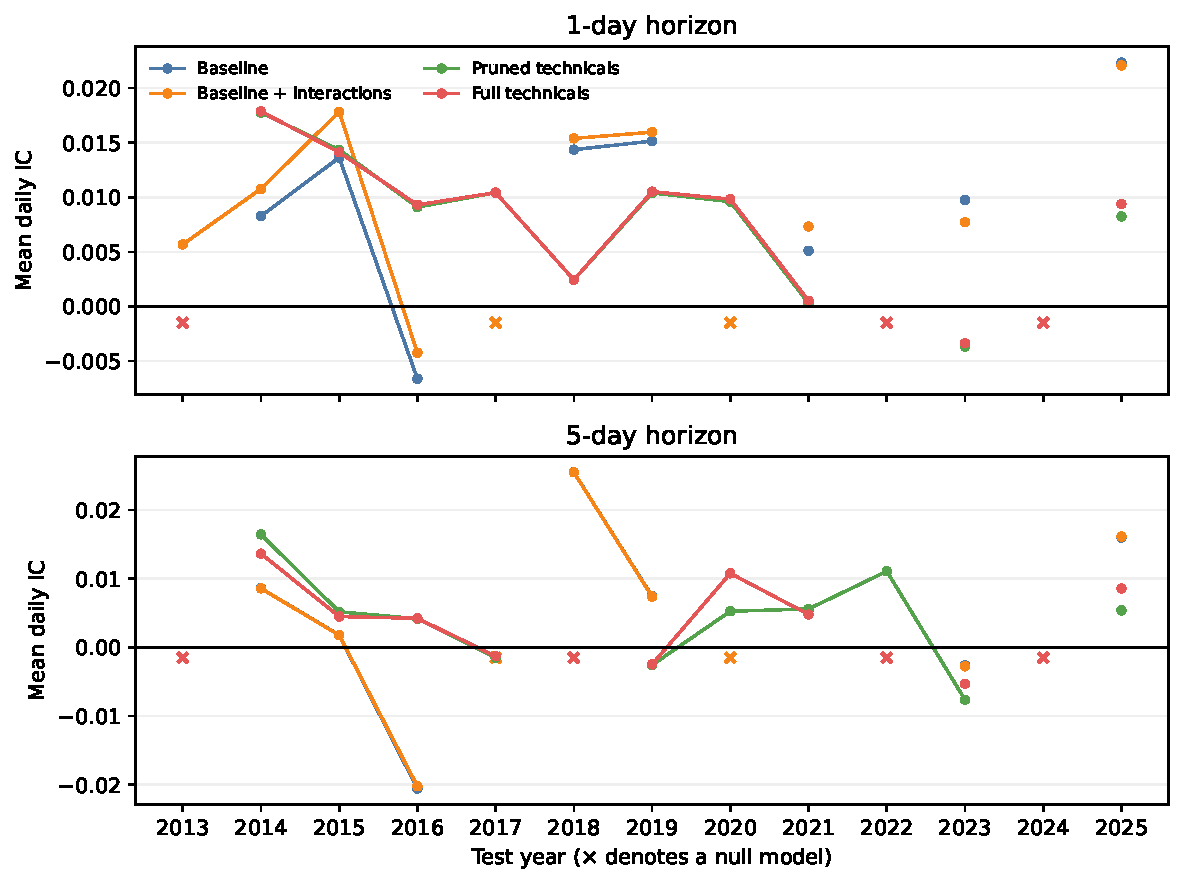
\includegraphics[width=0.88\textwidth]{yearly_ic.pdf}
\caption{Mean daily cross-sectional Spearman IC by test year. Lines stop at
null folds; crosses identify the corresponding years.}
\label{fig:yearly}
\end{figure}

The predeclared stress years reinforce the same pattern
(Appendix~\ref{app:stress}). The one-day pruned model is active with positive
IC in 2020 and 2025 and null in 2022. Its five-day counterpart is active in
all three years. Since each stress observation is a single test year, these
comparisons describe model behavior rather than establish a separate regime
effect.

\subsection{Cross-sectional portfolio sorts}

Figure~\ref{fig:deciles} averages the ten decile returns first within each
test year and then across active years. The shaded regions are 95\% intervals
based on variation in yearly means. One-day technical specifications separate
the two tails more clearly than the baseline. At five days, the baseline
ranking is almost flat and its highest predicted decile underperforms its
lowest. This explains how a positive full-cross-section IC can coexist with a
negative long-short spread.

\begin{figure}[ht]
\centering
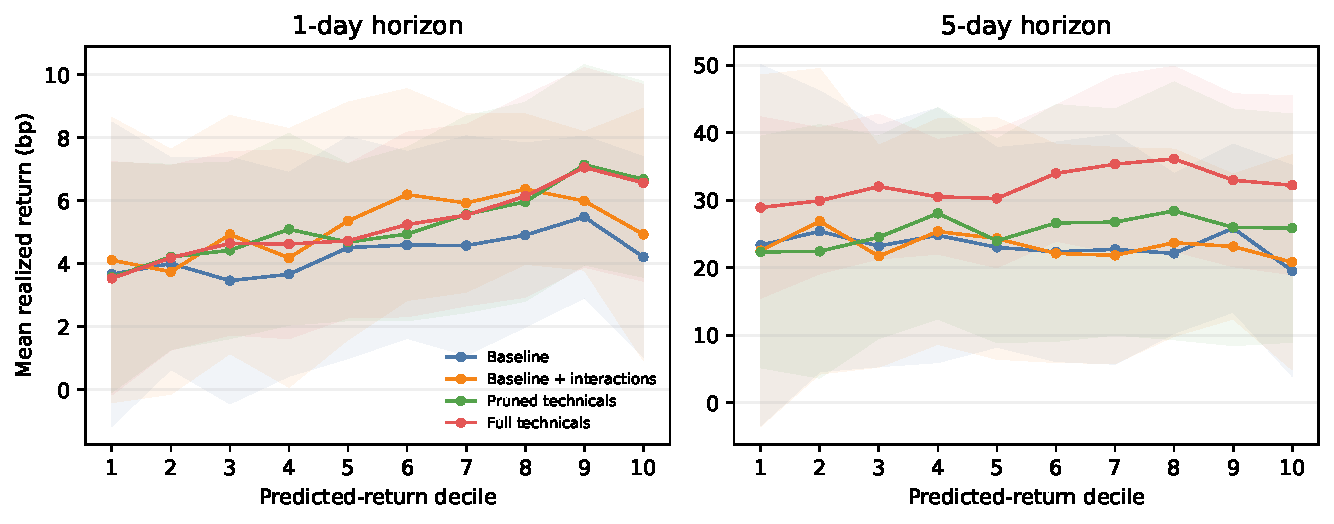
\includegraphics[width=0.94\textwidth]{decile_profiles.pdf}
\caption{Mean realized return by predicted-return decile. Bands are
$\pm1.96$ standard errors across annual means.}
\label{fig:deciles}
\end{figure}

\subsection{Selected signals and normalization}

The selected technical model changes materially across folds.
Figure~\ref{fig:coefs} shows the twelve largest average coefficient
magnitudes in the pruned specification. Range, reversal, and price-shape
signals recur, but their weights and active sets vary. The one-day 2021 fit
uses all 85 features; the five-day 2023 and 2025 fits use 85 and 83. These
dense fits sit beside years in which every coefficient is zero. The library
therefore behaves as a time-varying combination rather than a stable small
set of dominant formulas.

\begin{figure}[ht]
\centering
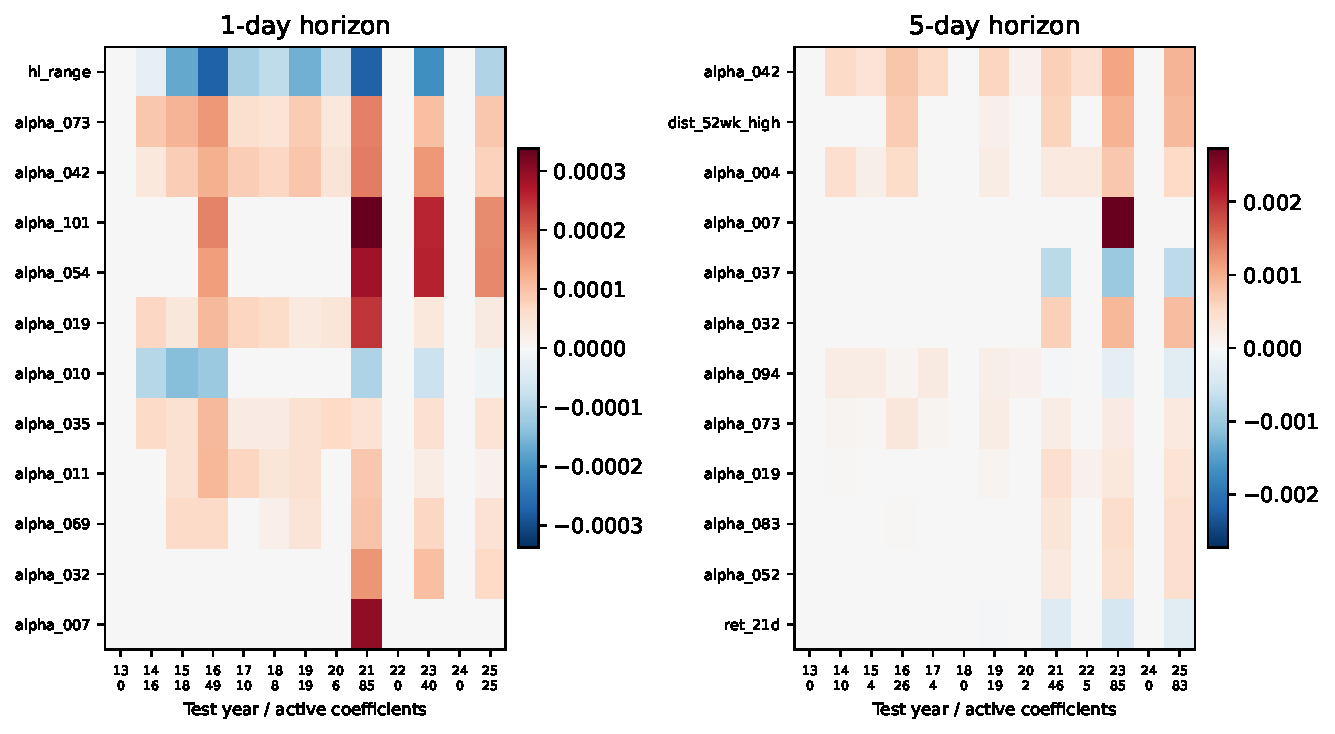
\includegraphics[width=0.94\textwidth]{coefficient_stability.pdf}
\caption{Elastic-net coefficients for the twelve largest average magnitudes
in the pruned technical model. The second line of each x-axis label gives the
number of active coefficients in that year.}
\label{fig:coefs}
\end{figure}

As a preprocessing sensitivity check, the baseline, pruned, and full models
were also estimated after within-fold winsorization and standardization.
Table~\ref{tab:normalization} compares only years in which both versions are
active. The similarity of the pruned and full models remains, while the sign
of the scaling effect differs between the baseline and technical
specifications. Rank normalization was the specified default; the ablation
shows that the magnitude of the technical result is sensitive to feature
scaling.

\begin{table}[ht]
\centering
\caption{One-day normalization ablation over paired active years.
$\Delta$ is standardized minus ranked mean daily-Spearman IC.}
\label{tab:normalization}
\small
\begin{tabular}{@{}lcccc@{}}
\toprule
Specification & Rank IC & Standardized IC & $\Delta$ & Paired years \\
\midrule
Baseline & 0.0087 & 0.0109 & 0.0022 & 5 \\
Pruned technicals & 0.0091 & 0.0035 & $-0.0057$ & 7 \\
Full technicals & 0.0092 & 0.0034 & $-0.0058$ & 7 \\
\bottomrule
\end{tabular}
\end{table}

\FloatBarrier
\section{Interpretation}

The experiments give different answers for the center of the cross-section
and its tails. Rank IC uses every security and rewards a broadly correct
ordering. The portfolio sort uses only two deciles. A forecast may organize
the middle of the cross-section while reversing its most extreme predictions,
or produce modest average ordering with useful tail separation. The
five-day baseline and one-day technical models illustrate these two cases.

The prune comparison is also informative. The frozen correlation rule reduces
the library by 17\% without materially changing out-of-sample results. It
removes obvious redundancy and lowers computation, while elastic net performs
the economically relevant target-aware selection inside each training fold.
The coefficient heatmap suggests that selection instability is a more
important feature of the experiment than the exact library size.

\subsection{Limitations}
\label{sec:limitations}

First, Equation~\eqref{eq:target} is a split-adjusted price return. Compounded
CRSP \texttt{ret} would include distributions and would follow the target
construction suggested in the project brief. Second, several signals use the
date-$t$ closing bar while the target begins at that close. The portfolio
interpretation therefore embeds a same-close execution convention; the IC
comparison is more defensible than the simulated trading return. Third,
transaction costs and turnover are absent. Daily decile rebalancing can make
a statistically positive spread economically unusable.

Fourth, the supplied course panel contains roughly 1{,}000 names per day, but
its point-in-time universe-membership construction cannot be independently
verified from this repository. Active-year IC averages condition on validation selecting a
nonconstant model. The all-fold column makes this conditioning visible, and
the annual plot retains null and negative years. Five-day Sharpe also depends
on the chosen non-overlapping formation offset; Appendix~\ref{app:offset}
reports the full range rather than selecting the best offset.

\section{Conclusion}

The broad technical specifications do not improve average cross-sectional
rank IC relative to the reversal/momentum benchmark, although they generate
greater one-day separation between the extreme deciles. Reducing the covered
library from 103 to 85 features leaves performance essentially unchanged,
consistent with elastic net absorbing much of the remaining redundancy.
These weak and time-varying results support the use of simple benchmarks,
yearly validation, and multiple evaluation metrics when studying technical
signals.

\begin{thebibliography}{9}
\bibitem{jegadeesh}
N.~Jegadeesh, ``Evidence of Predictable Behavior of Security Returns,''
\textit{Journal of Finance}, 45(3), 881--898, 1990.

\bibitem{lehmann}
B.~Lehmann, ``Fads, Martingales, and Market Efficiency,''
\textit{Quarterly Journal of Economics}, 105(1), 1--28, 1990.

\bibitem{kakushadze}
Z.~Kakushadze, ``101 Formulaic Alphas,'' \textit{Wilmott},
2016(84), 72--81, 2016.

\bibitem{zouhastie}
H.~Zou and T.~Hastie, ``Regularization and Variable Selection via the
Elastic Net,'' \textit{Journal of the Royal Statistical Society: Series B},
67(2), 301--320, 2005.
\end{thebibliography}

\clearpage
\appendix

\section{Data and feature audit}

\begin{table}[ht]
\centering
\caption{Panel audit used before report preparation.}
\small
\begin{tabular}{@{}lr@{}}
\toprule
Check & Result \\
\midrule
Rows after required-price filter & 6{,}253{,}895 \\
Unique securities / dates & 3{,}253 / 6{,}266 \\
Duplicate $(\texttt{permno},\texttt{date})$ keys & 0 \\
Rows removed for missing close or market cap & 1{,}180 (0.019\%) \\
Missing open & 0.069\% \\
Listing segments / gaps over 10 days & 8{,}748 / 5{,}495 \\
One-day target missing & 0.140\% \\
Five-day target missing & 0.699\% \\
\bottomrule
\end{tabular}
\end{table}

\texttt{alpha\_007} illustrates the difference between coverage and
variation. It is finite but equals $-1$ on 99.89\% of rows and is
cross-sectionally constant on 41.6\% of dates. The feature remains in the
frozen pruned list; elastic net decides whether it is active in each fold.

\section{Feature library}
\label{app:features}

\begin{sloppypar}
Skipped formulaic-alpha numbers are 48, 67, 90, and 100 (subindustry);
58, 76, and 79 (sector); and 59, 66, 82, and 89 (identities). The remaining
90 are implemented. The 15 classic features are
\texttt{oc\_ret}, \texttt{hl\_range}, \texttt{overnight\_gap},
\texttt{close\_loc}, \texttt{ret\_21d}, \texttt{mom\_63},
\texttt{mom\_6\_1}, \texttt{vol\_21d}, \texttt{parkinson\_vol\_21d},
\texttt{vol\_of\_vol\_63d}, \texttt{vol\_vs\_mean21},
\texttt{dollar\_vol\_rank}, \texttt{amihud\_21d},
\texttt{dist\_52wk\_high}, and \texttt{max\_ret\_21d}.
\end{sloppypar}

The correlation screen removes \texttt{alpha\_096} and
\texttt{alpha\_097} for coverage, then retains 85 of 103 features at
$|\rho|=0.7$. Figure~\ref{fig:prune} displays the frozen-sample matrix.

\begin{figure}[ht]
\centering
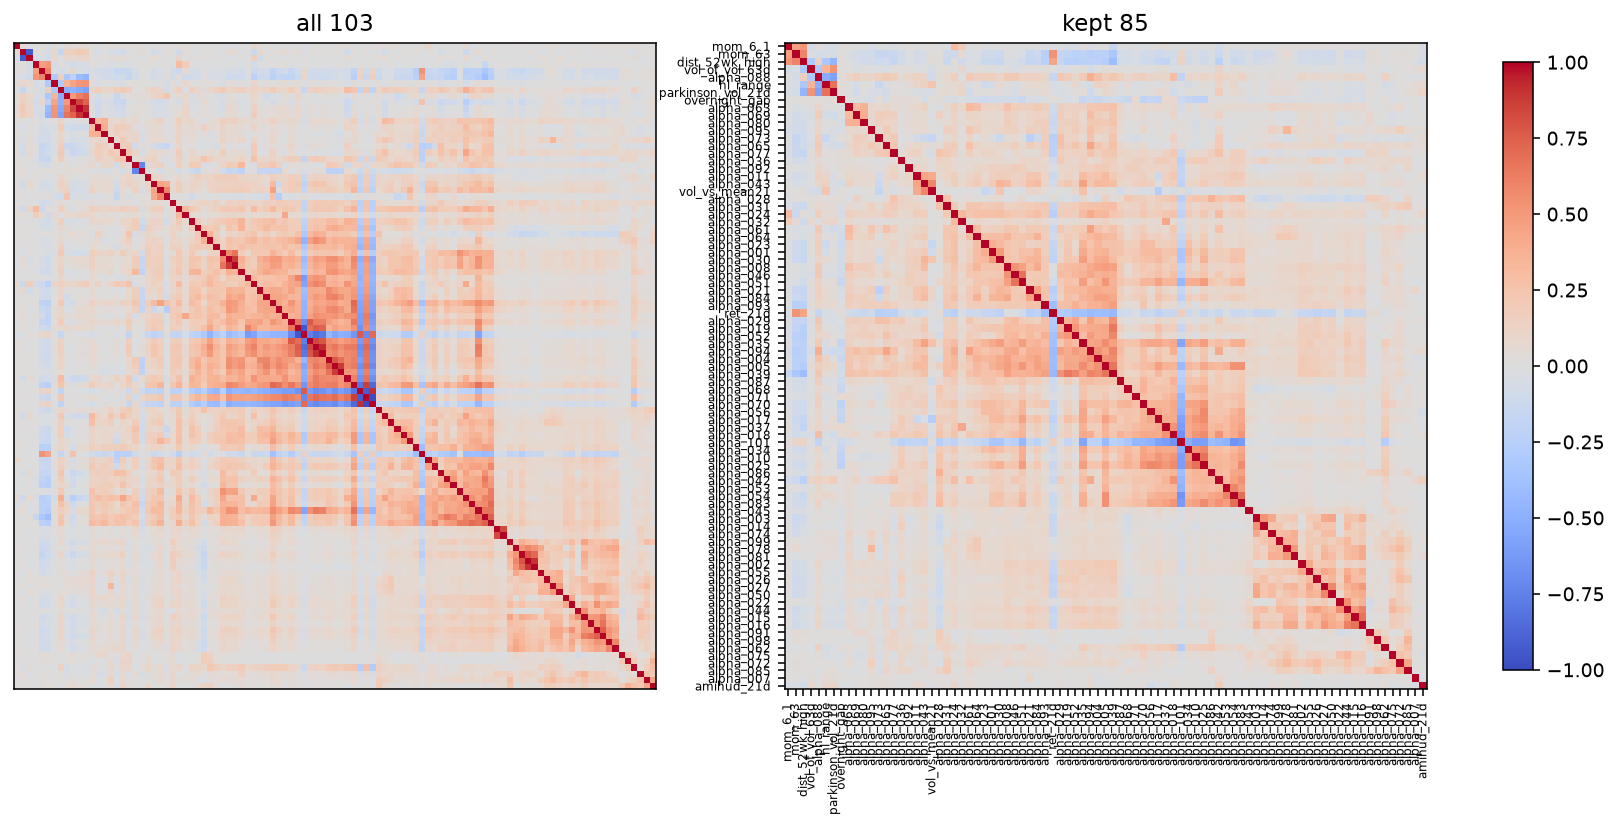
\includegraphics[width=0.92\textwidth]{prune_corr.png}
\caption{Mean daily Spearman correlations in the 2001--2010 pruning sample,
before and after the $|\rho|=0.7$ filter.}
\label{fig:prune}
\end{figure}

\section{Tuning diagnostics}

\begin{figure}[ht]
\centering
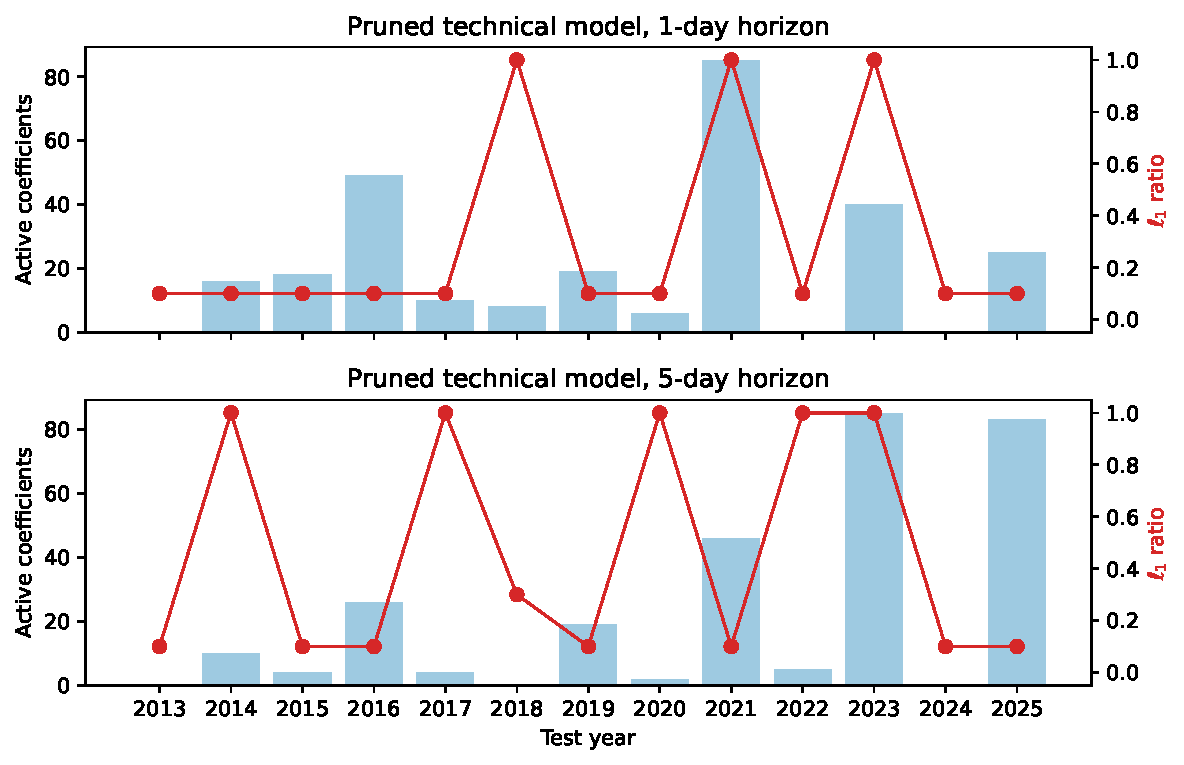
\includegraphics[width=0.86\textwidth]{tuning_complexity.pdf}
\caption{Selected $\ell_1$ ratio and active-set size for the pruned technical
model. Parameters are chosen on the preceding validation year.}
\label{fig:tuning}
\end{figure}

Raw $\alpha$ values are not directly comparable across folds because each
path is scaled by its training-derived $\alpha_{\max}$. The active-set size
shows the effective complexity. For the one-day pruned model, validation
selects zero coefficients in 2013, 2022, and 2024 and all 85 in 2021. At the
five-day horizon, 2013, 2018, and 2024 are null, while 2023 and 2025 retain
85 and 83 features.

\section{Stress-year results}
\label{app:stress}

\begin{table}[ht]
\centering
\caption{Predeclared stress years. Entries are annual mean daily IC and gross
Sharpe. Dashes identify null folds.}
\small
\begin{tabular}{@{}lccccccc@{}}
\toprule
 & & \multicolumn{2}{c}{2020} & \multicolumn{2}{c}{2022}
 & \multicolumn{2}{c}{2025} \\
\cmidrule(lr){3-4}\cmidrule(lr){5-6}\cmidrule(lr){7-8}
Specification & $h$ & IC & SR & IC & SR & IC & SR \\
\midrule
Baseline & 1d & --- & --- & --- & --- & 0.022 & 0.51 \\
Baseline & 5d & --- & --- & --- & --- & 0.016 & 0.57 \\
Pruned technicals & 1d & 0.010 & 0.72 & --- & --- & 0.008 & 0.25 \\
Pruned technicals & 5d & 0.005 & 0.51 & 0.011 & 0.21 & 0.005 & 0.24 \\
\bottomrule
\end{tabular}
\end{table}

\section{Five-day formation-offset sensitivity}
\label{app:offset}

Table~\ref{tab:offsets} summarizes, for each specification, the five
possible non-overlapping five-day formation series.

\begin{table}[ht]
\centering
\caption{Five-day results across all non-overlapping formation offsets.
Spread is the 100\%-gross return in basis points per five-day period.}
\label{tab:offsets}
\small
\begin{tabular}{@{}lccccc@{}}
\toprule
Specification & Min SR & Median SR & Max SR & Min spread & Max spread \\
\midrule
Baseline & $-0.15$ & $-0.00$ & 0.16 & $-2.51$ & 2.81 \\
Baseline + interactions & $-0.16$ & $-0.03$ & 0.19 & $-2.68$ & 3.39 \\
Pruned technicals & 0.12 & 0.38 & 0.72 & 1.78 & 11.86 \\
Full technicals & 0.11 & 0.34 & 0.64 & 1.67 & 10.95 \\
\bottomrule
\end{tabular}
\end{table}

\FloatBarrier
\section{Reproducibility}

\begin{sloppypar}
The main experiment is run from the repository root with
\texttt{uv run python run\_models.py}. The normalization ablation behind
Table~\ref{tab:normalization} is reproduced by
\texttt{uv run python run\_normalization\_ablation.py}, which refits the
one-day models under both schemes and rewrites its summary CSV under
\texttt{outputs/ablation\_normalization/}. Report tables and figures are
then generated by \texttt{uv run python run\_report\_figures.py}. The panel
audit is reproduced by \texttt{uv run python run\_panel\_audit.py}. The
small CSVs under \texttt{outputs/report/} support the model exhibits; the
data-audit table comes from \texttt{outputs/panel\_audit.json}. The
course-provided raw panel and large prediction files are not versioned; full
regeneration therefore requires access to the course data.
\end{sloppypar}

\end{document}
